\documentclass{article}
\usepackage[utf8]{inputenc}
\usepackage{polski}
\usepackage{amsmath}
\usepackage{titlesec}
\usepackage[labelsep=period]{caption}
\usepackage{graphicx}

\titlelabel{\thetitle.\quad}

\title{Sprawozdanie z zadania P3.4\\- zastosowanie metod numerycznych do zmiany rozmiaru obrazów}
\author{Aleksander Czeszejko-Sochacki\\Sławomir Górawski}
\date{28 stycznia 2018}

\begin{document}

\maketitle

\section{Wstęp}

Zmiana rozmiaru obrazu to jedna z najczęściej wykonywanych operacji w grafice komputerowej. Pomijając zagadnienia związane z kompresją, każdy czarno-biały obraz można potraktować jak bitmapę, tj. macierz liczb odpowiadających odcieniom poszczególnych pikseli, o rozmiarze takim, jak rozmiar obrazu. Liczby te mogą być całkowite, z przedziału [0, 255], lub zmiennoprzecinkowe, z przedziału [0, 1]. W obu przypadkach ich wielkość jest wprost proporcjonalna do jasności danych pikseli, zatem w przypadku liczb typu \textit{float} 0 oznacza piksel całkowicie czarny, a 1 - całkowicie biały.

Wynika z tego, że obraz o rozmiarze $x\times y$ jest opisany przez $x\cdot y$ liczb. Jeśli chcemy go powiększyć, musimy wiedzieć, jaki odcień mają mieć nowe piksele. Ich dokładnej wartości, rzecz jasna, nie znamy. Możemy je jednak przybliżać przy użyciu algorytmów bazujących na metodach numerycznych. Trzy z nich zostały omówione, zaimplementowane i przetestowane.

\section{Krótki opis algorytmów}

Wszystkie algorytmy przedstawione poniżej ograniczają się do działania na wektorach o długości $M$, tj. w jednym wymiarze. Aby używać ich na obrazach, bitmapę można traktować jako zbiór wektorów kolumnowych i skalować każdy z nich po kolei, co poskutkuje zmianą wysokości całego obrazu. Aby zmienić również szerokość obrazu, można go transponować i powtórzyć działanie. Taka procedura umożliwia zmianę rozmiaru obrazu w dwóch wymiarach przy użyciu dowolnego z poniższych algorytmów. Wartości odcieni nowych pikseli będziemy obliczać w punktach $p_i$ ($N$ -- nowy rozmiar obrazu):

$$p_i = 1 + (i - 1)\tfrac{M-1}{N-1} \quad \text{dla} \quad i = 1, 2, \dots, N.$$

\subsection{Metoda najbliższego sąsiedztwa}

W tej metodzie każdy nowy piksel przyjmuje odcień $K$ tego, który miał najbliższy indeks przed skalowaniem. Można to wyrazić wzorem:

$$K(p_i) = K(\text{round}(p_i)) \quad \text{dla} \quad i = 1, 2, \dots, N.$$

Warto zauważyć, że w tej metodzie pojawiają się wyłącznie wartości dane na wejściu - nie ma miejsce generowanie żadnych nowych liczb. W teorii zatem powiększony obraz nie powinien wyglądać w żaden sposób lepiej od wyjściowego, ale z kolei przy pomniejszaniu może to nie mieć większego znaczenia, a może nawet być zaletą.

\subsection{Metoda bazująca na interpolacji funkcją sklejaną pierwszego stopnia}

Ten algorytm polega na konstrukcji funkcji sklejanej pierwszego stopnia, której węzły stanowią piksele obrazu przed skalowaniem:

$$S(t_i) = K(t_i) \quad \text{dla} \quad i = 1, 2, \dots, M.$$

Można o tym myśleć jak o łamanej złożonej z odcinków łączących wartości tych pikseli. Wartości pikseli w nowym obrazie będą równe wartości funkcji sklejanej w tych punktach:

$$K(p_i) = S(p_i) \quad \text{dla} \quad i = 1, 2, \dots, N.$$

\subsection{Metoda bazująca na interpolacji naturalną funkcją sklejaną trzeciego stopnia}

Jeżeli specyfikacja zadania umożliwia zastosowanie w nim funkcji sklejanej pierwszego stopnia, to naturalnym pomysłem jest rozważenie również interpolacji splajnem trzeciego stopnia, który dla tych samych danych jest zwykle w stanie zapewnić dokładniejsze przybliżenie. Działanie algorytmu wygląda podobnie jak poprzednio:

\begin{align*}
    Z(t_i) = K(t_i) \quad &\text{dla} \quad i = 1, 2, \dots, M,\\
    K(p_i) = Z(p_i) \quad &\text{dla} \quad i = 1, 2, \dots, N.
\end{align*}

\section{Cel wykonanych doświadczeń}

Celem zadania było przetestowanie w praktyce działania powyższych algorytmów oraz ich porównanie. W przypadku skalowania obrazów ciężko o konkretny wskaźnik poprawności czy też błędu, jednakże po zestawieniu obok siebie obrazów otrzymanych po przekształceniu tego samego obrazu źródłowego testowanymi algorytmami można łatwo dojść do kilku wniosków dotyczących własności tego przekształcenia.

Oprócz jakości obrazów po zmianie rozmiaru testowane były również czasy działania poszczególnych algorytmów oraz to, czy kolejność kierunków skalowania ma znaczenie (można to robić najpierw w pionie, a potem w poziomie, lub na odwrót). W celu oceny tego ostatniego tworzone były obrazy różnicy, powstałe w następujący sposób:

$$D(\cdot,\cdot) = 1 - |K^{(1)}(\cdot,\cdot) - K^{(2)}(\cdot,\cdot)|.$$

Ciemniejsze obszary na obrazie D oznaczały miejsca, w których obrazy przeskalowane sposobami (1) i (2) różniły się w sposób znaczący.

\section{Opis użytych metod}

W pliku \texttt{program.jl} zaimplementowane zostały funkcje bazujące na opisanych algorytmach, zmieniające wysokość obrazu, iterując po jego kolumnach (ze względu na specyfikę języka \textbf{Julia} jest to znacznie szybsze od iteracji po rzędach). Do pełnej zmiany rozmiaru obrazu służy funkcja \texttt{resize}, przyjmująca jako parametry: obraz, nowe wymiary, metodę zmiany jego rozmiaru oraz kierunek, w jakim ma zostać przeprowadzone pierwsze skalowanie (dwa ostatnie parametry mają postać enumeratorów utworzonych przy pomocy makra \texttt{@enum}).  

Funkcja \texttt{resize} w celu zmiany rozmiaru obrazu skaluje go w jednym kierunku, transponuje go, skaluje w drugim kierunku, i zwraca ponownie transponowany wynik. Domyślnie zmiana rozmiaru odbywa się najpierw w pionie, potem w poziomie, jednak jeśli sprecyzowano inaczej, odwrotna kolejność osiągnięta zostaje przez kolejne dwie transpozycje: przed rozpoczęciem skalowania w obu kierunkach i po jego zakończeniu.

Do testowania użyto bibliotek: \textbf{Images}, umożliwiającej przeprowadzanie wielu operacji na obrazach, \textbf{TestImages}, zapewniającej wygodny dostęp do standardowych obrazów testowych oraz \textbf{PyPlot}, w celu prezentacji wyników. Jakość poszczególnych przekształceń zaprezentowana została przez zestawienie obok siebie obrazów otrzymanych przez zastosowanie poszczególnych algorytmów, czasy działania zostały zmierzone przy użyciu makra \texttt{@elapsed}, działającego podobnie do \texttt{@time}, z kolei znaczenie kolejności kierunków pokazane zostało na opisanych wcześniej obrazach różnicy.

\newpage
\section{Opis wykonanych doświadczeń}

\subsection{Powiększanie obrazu}

Pierwsze doświadczenie polegało na dwukrotnym zwiększeniu rozmiaru czarno-białego zdjęcia. Otrzymane wyniki:

\begin{figure}[ht]
    \centering
    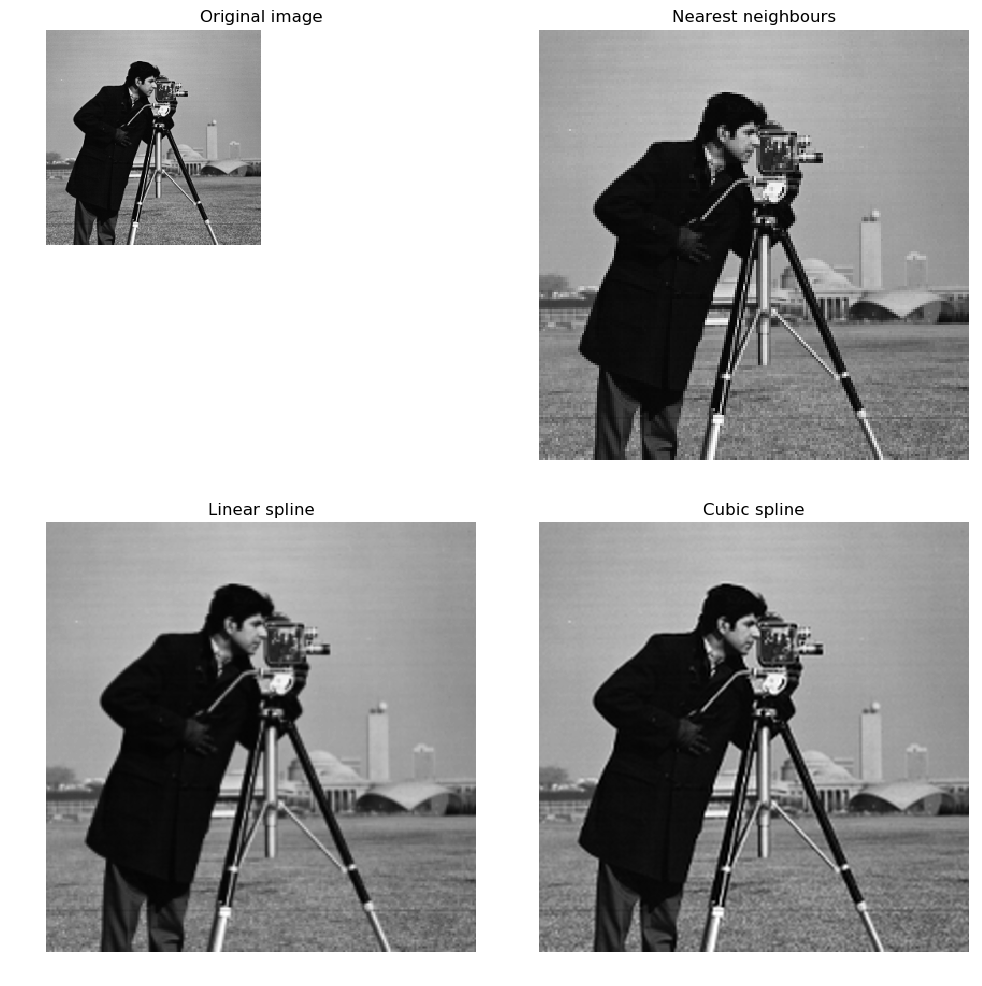
\includegraphics[width=\textwidth]{images/cameraman-com.png}
    \caption{Porównanie algorytmów przy powiększaniu}
    \label{fig:cameraman-com}
\end{figure}

Można łatwo zaobserwować, że obraz po przekształceniu \textit{metodą najbliższego sąsiedztwa} nie wygląda w żaden sposób lepiej od źródłowego - zajmuje tylko więcej miejsca. Zgodnie z oczekiwaniami zatem metoda ta nie jest dobra do zwiększania rozmiaru. Skalowanie bazujące na interpolacji funkcją sklejaną pierwszego stopnia daje znacznie lepszy pod tym względem wynik, jednak obraz po przekształceniu wygląda na nieco nieostry. Algorytm wykorzystujący splajn trzeciego stopnia zdecydowanie wygrywa całe porównanie, zwracając tak samo gładki, jednak jednocześnie ostrzejszy obraz -- najlepiej odwzorowujący pierwowzór.

\begin{table}[ht]
    \centering
    \begin{tabular}{|l|r|}
        \hline
        \textit{metoda najbliższego sąsiedztwa} & 0,030154s \\
        splajn pierwszego stopnia & 0,011554s \\
        splajn trzeciego stopnia & 0,792738s \\
        \hline
    \end{tabular}
    \caption{Porównanie czasów działania przy powiększaniu}
    \label{tab:cameraman-times}
\end{table}

Pomiar czasu przy użyciu makra \texttt{@elapsed} nie jest zbyt precyzyjny, a jego wyniki zmieniają się z każdym wywołaniem (dla tych samych danych, oczywiście), jednak pozwala oszacować rzędy wielkości. Z tego przykładowego pomiaru, oraz innych, przeprowadzonych dla innych wywołań bądź przykładów, można wnioskować, że zarówno \textit{metoda najbliższego sąsiedztwa}, jak i ta bazująca na splajnie pierwszego stopnia działają w podobnym czasie, natomiast metoda oparta o interpolację naturalną funkcją sklejaną trzeciego stopnia jest zwykle ok. 10 razy wolniejsza. Patrząc na ilość obliczeń wymaganych do znalezienia współczynników splajna nie jest to szczególnie zaskakujące.

Z kolei kolejność kierunków skalowania w przypadku \textit{metody najbliższego sąsiedztwa} nie ma, rzecz jasna, znaczenia (jak było wspomniane, nie pojawiają się tu żadne nowe wartości, zatem jedynym ewentualnym źródłem różnic mogłyby być różnice zaokrągleń, czego nie udało się zaobserwować). W przypadku metod bazujących na splajnach da się jednak zaobserwować pewne różnice:

\begin{figure}[ht]
    \centering
    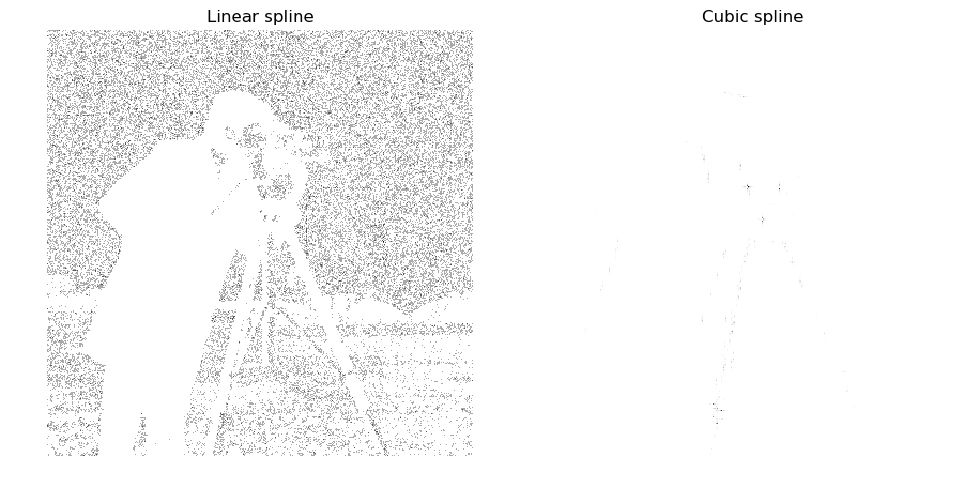
\includegraphics[width=\textwidth]{images/cameraman-diff.png}
    \caption{Obrazy różnicy dla zmiany kolejności kierunków skalowania}
    \label{fig:cameraman-diff}
\end{figure}

Jak widać, w przypadku skalowania liniowym splajnem różnice bywają dosyć znaczne, nie na jednolitych kolorystycznie obszarach (czarna sylwetka fotografa), ale na tych, gdzie kolor się zmienia na małym obszarze. W metodzie bazującej na naturalnej funkcji sklejanej trzeciego stopnia również istnieją pewne różnice, jednak ciężko je w ogóle zauważyć, zatem można je uznać w tym przypadku za pomijalne.

\subsection{Zmniejszanie obrazu}

Kolejny test polegał na porównaniu wyników zmniejszania zdjęcia:

\begin{figure}[ht]
    \centering
    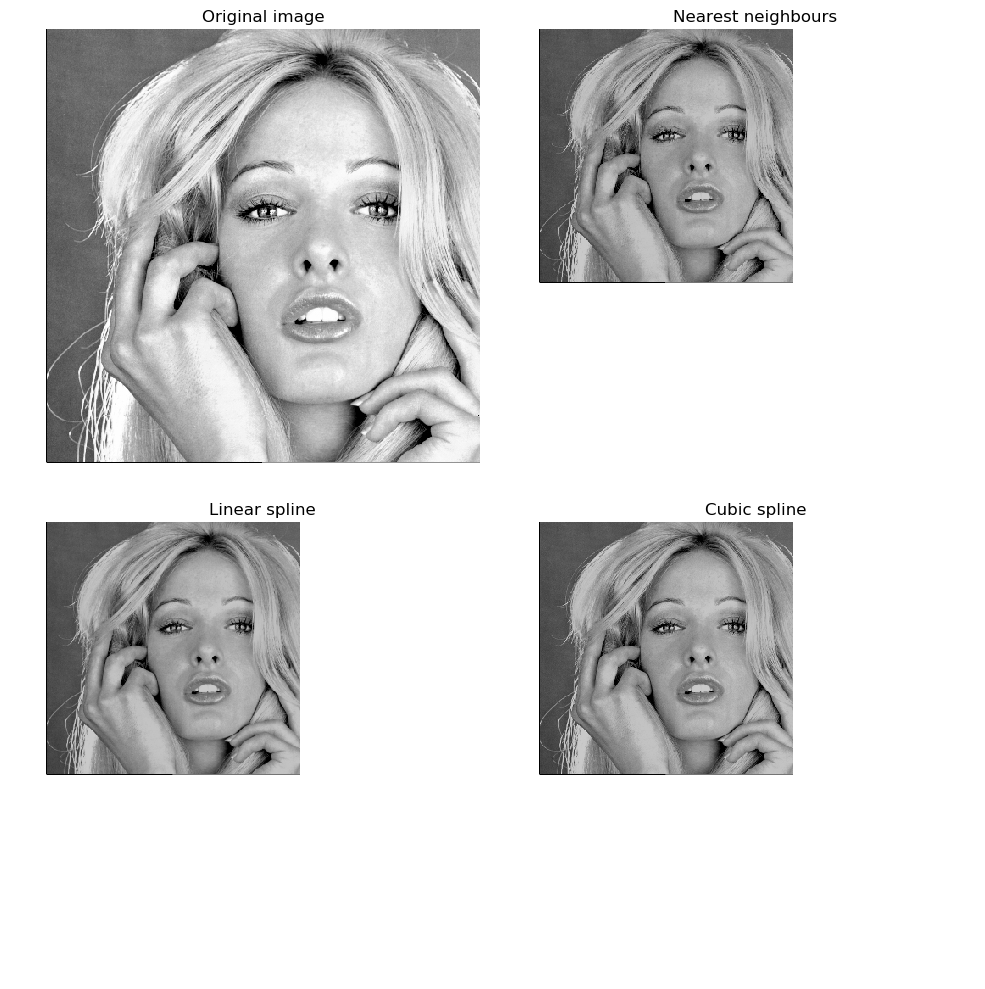
\includegraphics[width=\textwidth]{images/woman-com.png}
    \caption{Porównanie algorytmów przy zmniejszaniu}
    \label{fig:woman-com}
\end{figure}

Tutaj już przewaga jednej metody nad inną nie wydaje się taka oczywista - przede wszystkim obraz uzyskany \textit{metodą najbliższego sąsiedztwa} nie wygląda aż tak źle. Po zastanowieniu się prawdopodobnie dojdzie się do wniosku, że i tutaj splajn trzeciego stopnia wypada najlepiej, jednak jest to okupione jeszcze większą niż poprzednio różnicą czasów działania. Jeżeli chodzi o obrazy różnicy, to wyglądają podobnie, jak w poprzednim przykładzie.

\begin{table}[ht]
    \centering
    \begin{tabular}{|l|r|}
        \hline
        \textit{metoda najbliższego sąsiedztwa} & 0,019970s \\
        splajn pierwszego stopnia & 0,010779s \\
        splajn trzeciego stopnia & 1,642014s \\
        \hline
    \end{tabular}
    \caption{Porównanie czasów działania przy zmniejszaniu}
    \label{tab:woman-times}
\end{table}

\subsection{Deformacja obrazu}

Trzeci eksperyment polegał na deformacji obrazu, czyli zmniejszeniu go w jednym wymiarze i zwiększeniu w drugim. Zestawienie wizualne rezultatów nie jest szczególnie ciekawe i powiela wnioski z poprzednich testów; można je zobaczyć w pliku \texttt{program.ipynb} lub \texttt{program.html}. Warto jednak spojrzeć na obrazy różnicy:

\begin{figure}[ht]
    \centering
    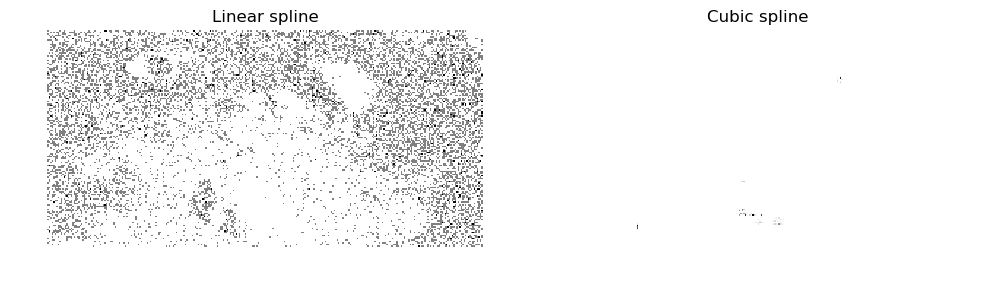
\includegraphics[width=\textwidth]{images/moon-diff.png}
    \caption{Obrazy różnicy}
    \label{fig:moon-diff}
\end{figure}

W przypadku deformacji przy użyciu funkcji sklejanej pierwszego stopnia można zaobserwować już znaczną różnicę. Splajn trzeciego stopnia wydaje się wciąż radzić z tym dobrze.

\subsection{Mocno kontrastowy obraz}

Aby móc spojrzeć na wyniki z nieco innej perspektywy, uwzględniony został też bardzo szczególny przypadek testowy, tj. szachownica. Jako obraz, na którym występują bardzo duże lokalne zmiany odcieni mógł on się okazać trudny dla metod, które lepiej radziły sobie ze zdjęciami:

\begin{figure}[ht]
    \centering
    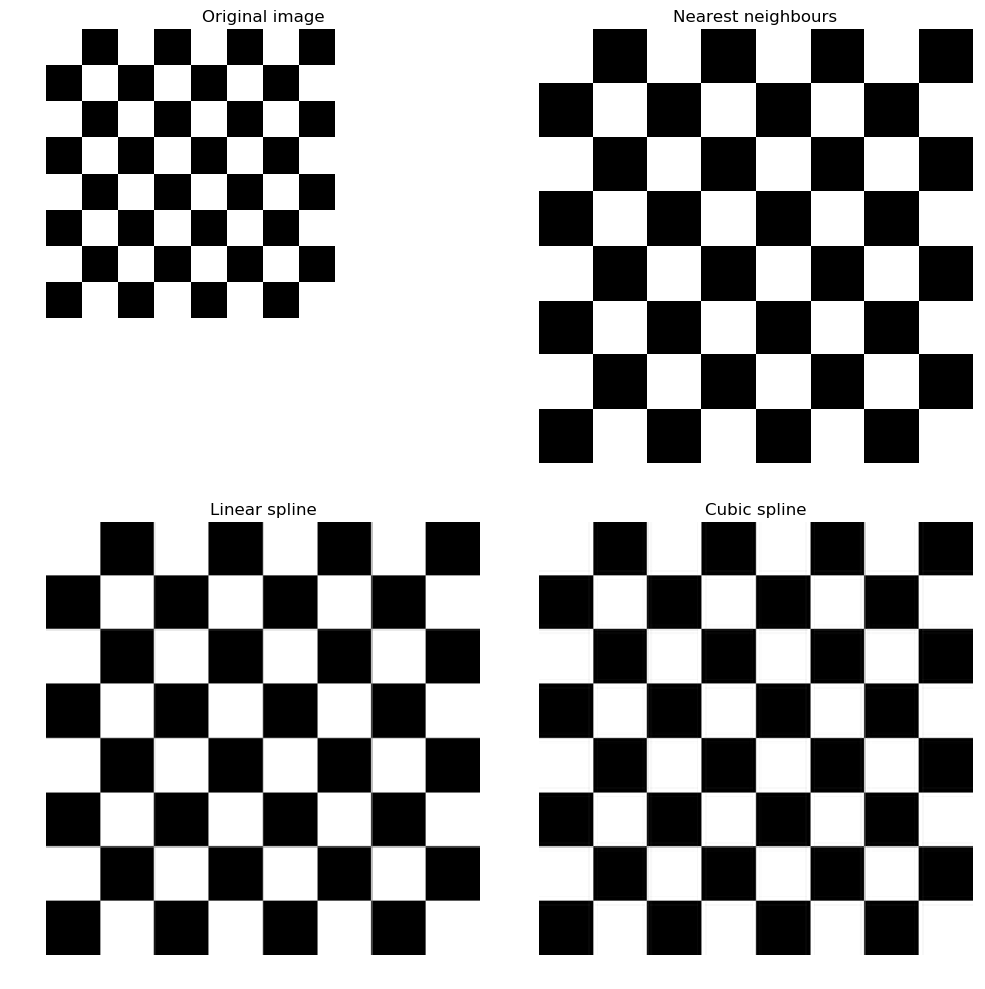
\includegraphics[width=\textwidth]{images/chessboard-com.png}
    \caption{Działanie metod dla mocno kontrastowego obrazu}
    \label{fig:chessboard-com}
\end{figure}

W tym przypadku, zgodnie z oczekiwaniami, tylko \textit{metodzie najbliższego sąsiedztwa} udało się dokładnie oddać pierwowzór. W przypadku metod bazujących na interpolacji widoczne są szare linie, które powodują, że obraz wydaje się rozmyty. Nie rzutuje to oczywiście na przewagę tychże metod w większości realnych zastosowań, jednak w pewnych szczególnych przypadkach podobnych do tego może mieć znaczenie.

\section{Wnioski}

Biorąc pod uwagę wyniki wszystkich testów, można wyciągnąć następujące wnioski:

\begin{itemize}
    \item do powiększania obrazów najlepiej nadaje się metoda bazująca na interpolacji naturalną funkcją sklejaną trzeciego stopnia,
    \item \textit{metoda najbliższego sąsiedztwa} oraz metoda bazująca na linowym splajnie działają w podobnym czasie, metoda bazująca na splajnie trzeciego stopnia jest znacznie wolniejsza,
    \item przy zmniejszaniu obrazów przewaga ostatniej metody nie jest aż tak widoczna, z kolei jeszcze bardziej odstaje ona pod względem czasu działania -- jeśli obraz ma być mały, można tu rozważyć zastąpienie jej np. splajnem liniowym,
    \item kolejność kierunków skalowania ma znaczenie w praktyce tylko w metodzie bazującej na funkcji sklejanej pierwszego stopnia -- największe, gdy obraz jest zmniejszany w jednym, a zwiększany w drugim wymiarze,
    \item w pewnych szczególnych przypadkach, gdy bardzo ważne jest zachowanie kontrastu, można rozważyć zastosowanie \textit{metody najbliższego sąsiedztwa}, gdyż ta jako jednyna nie rozmywa obrazu.
\end{itemize}

\end{document}
